\section{Introduction}

\label{sec:intro}

\begin{frame}{Problem statement}
	\only<1>
	{
	\vfill
	\begin{figure}
		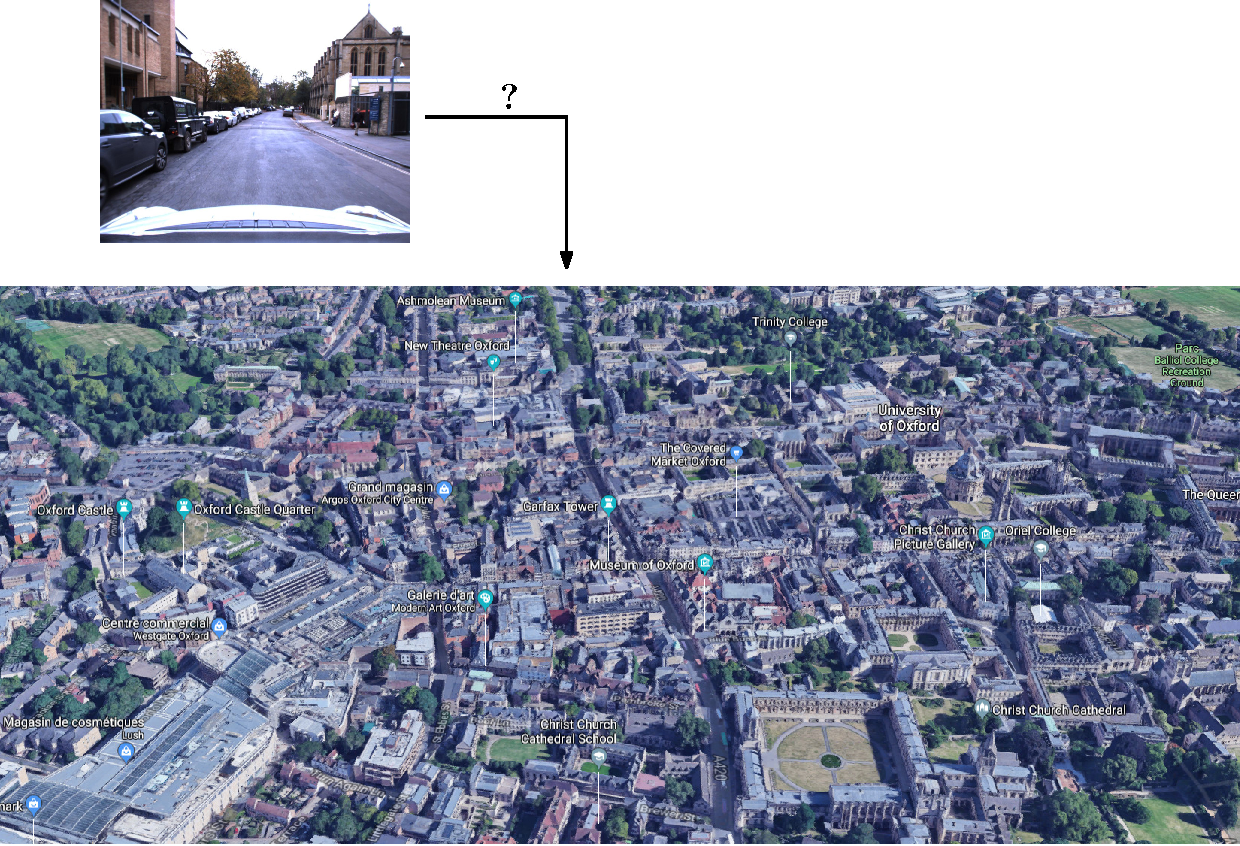
\includegraphics[width=0.8\linewidth]{vect/intro/fig1/1}
	\end{figure}
	\vfill	
	We aim to recover the position of an \textbf{unknown query}.
	}
	\only<2>
	{
	\vfill
	\begin{figure}
		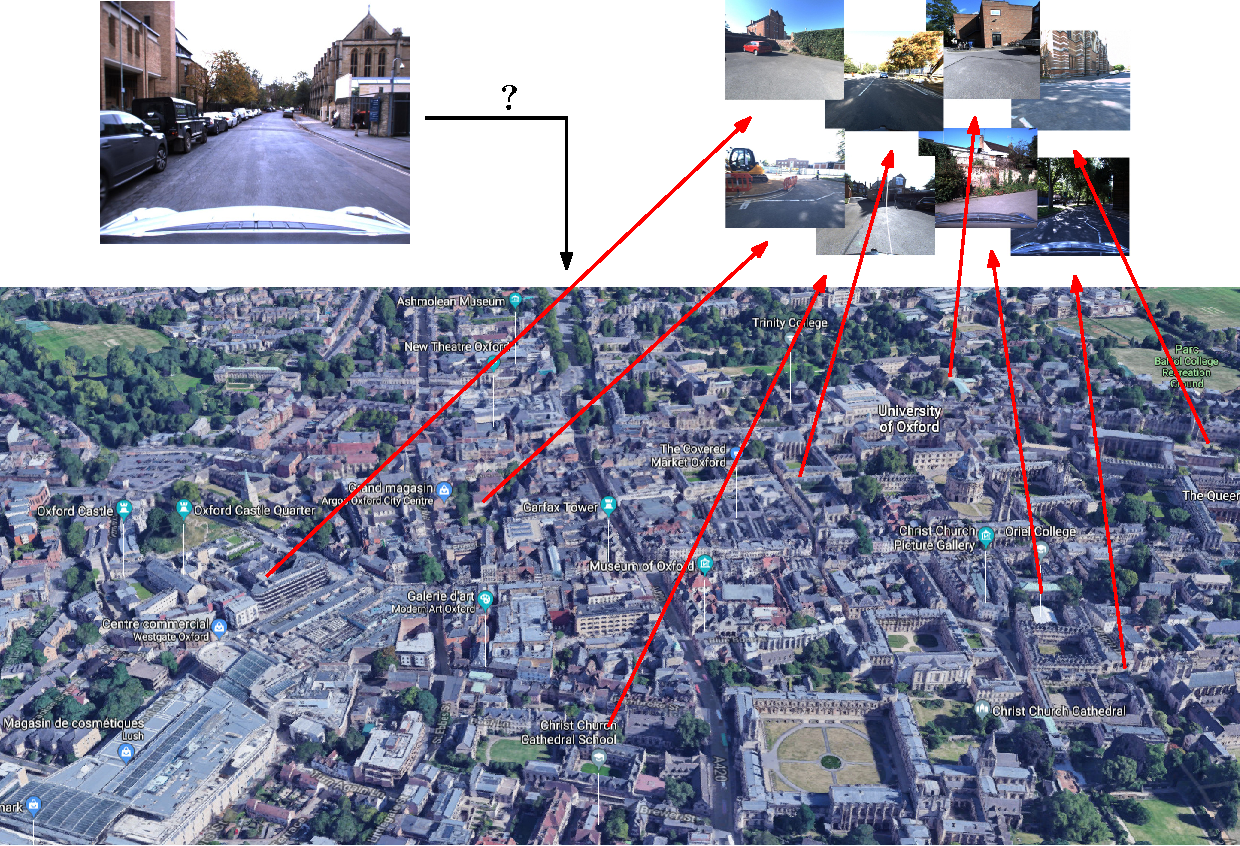
\includegraphics[width=0.8\linewidth]{vect/intro/fig1/2}
	\end{figure}
	\vfill	
	We have access to \textbf{geo-localized data}.
	}
	\only<3>
	{
	\vfill
	\begin{figure}
		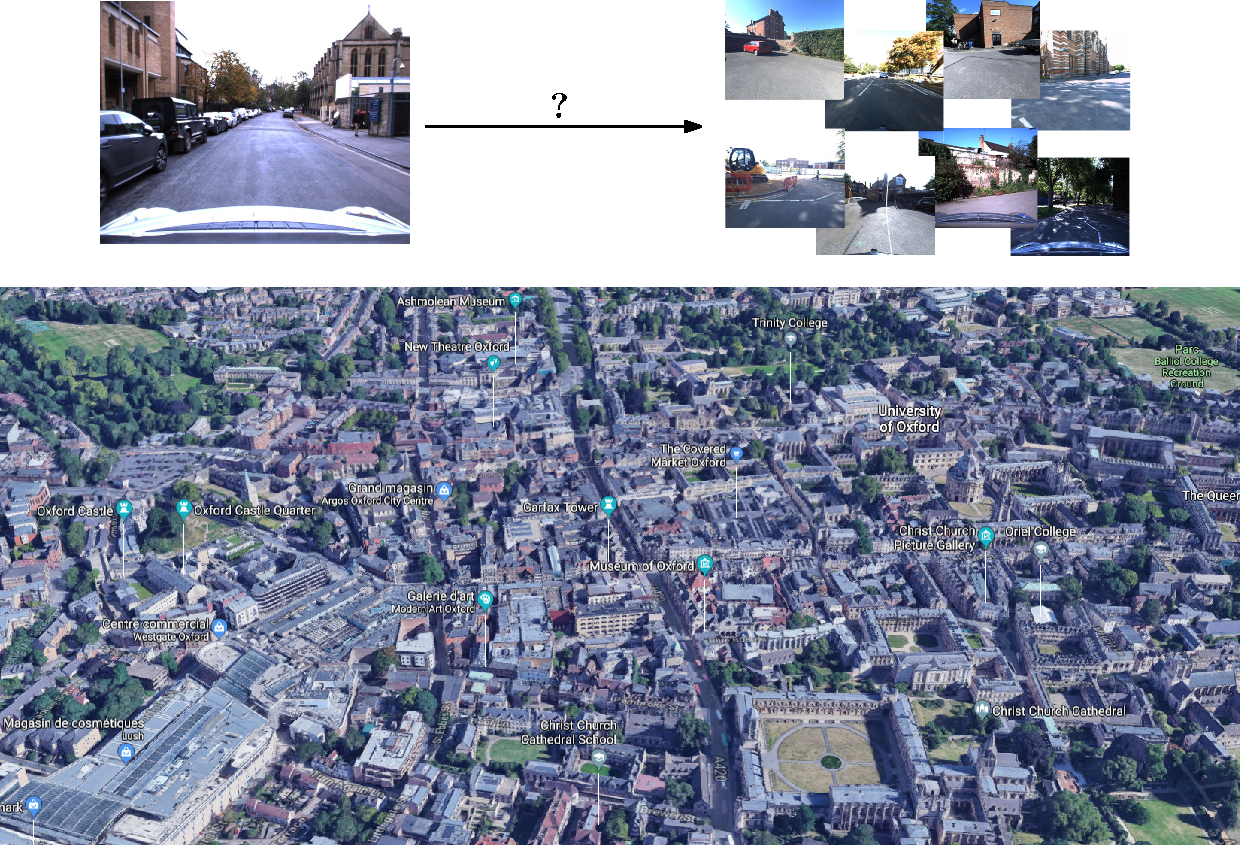
\includegraphics[width=0.8\linewidth]{vect/intro/fig1/3}
	\end{figure}
	\vfill	
	We caste the image localisation problem as an \textbf{image-retrieval problem}.
	}
	\only<4>
	{
	\vfill
	\begin{figure}
		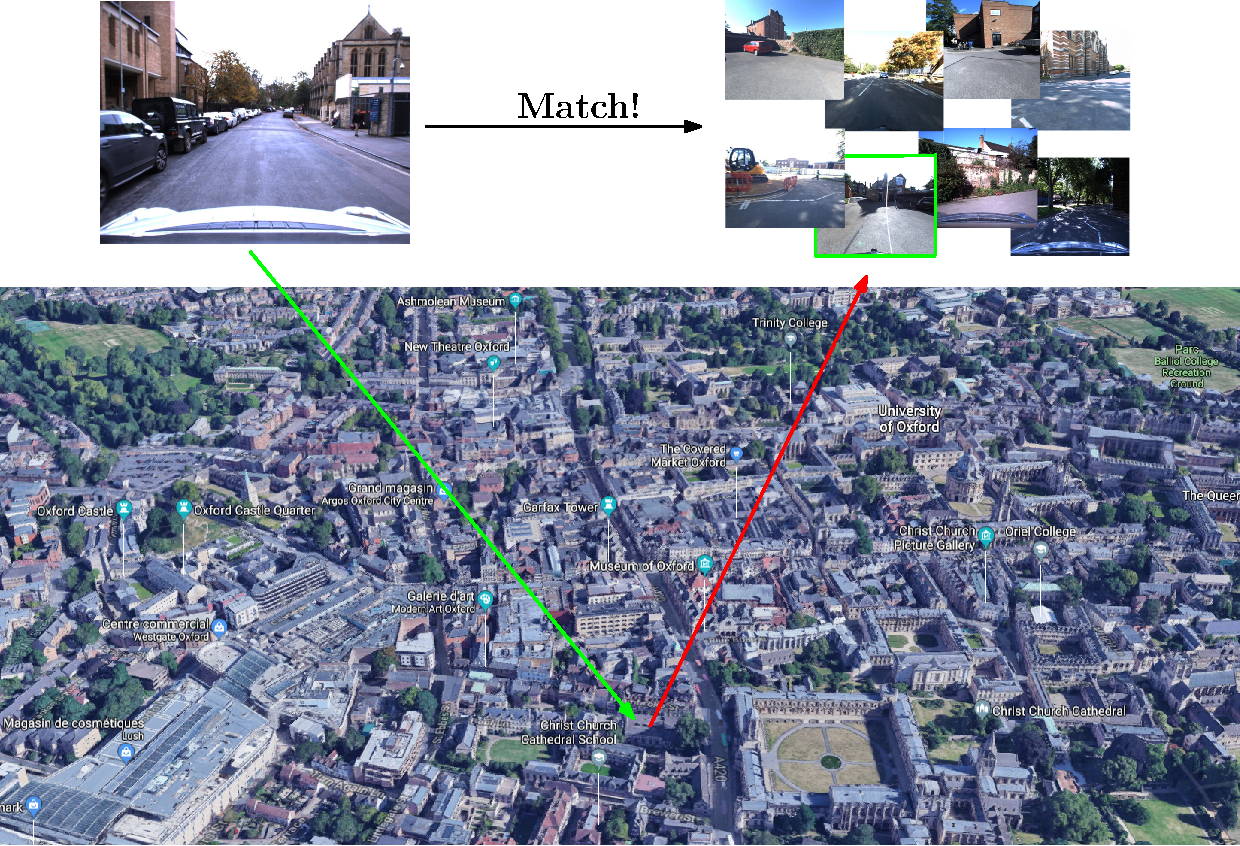
\includegraphics[width=0.8\linewidth]{vect/intro/fig1/4}
	\end{figure}
	\vfill	
	We transfer the position of the \textbf{retrieved candidate} to the query.
	}
\end{frame}

\begin{frame}{Applications}
	Visual based localization can be used in various situation:
	\vfill
	{\centering
	\begin{minipage}[t]{0.31\linewidth}
		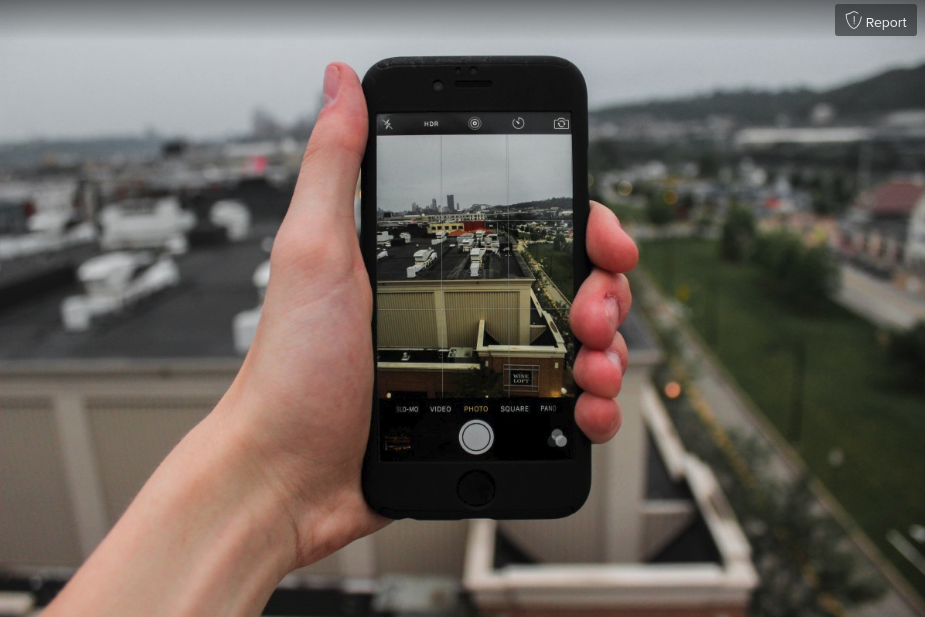
\includegraphics[width=\linewidth]{vect/intro/fig2/urban-loc}
		\vfill
		\textbf<1>{Pedestrian localization}
	\end{minipage}
	\uncover<2->{
	\begin{minipage}[t]{0.31\linewidth}
		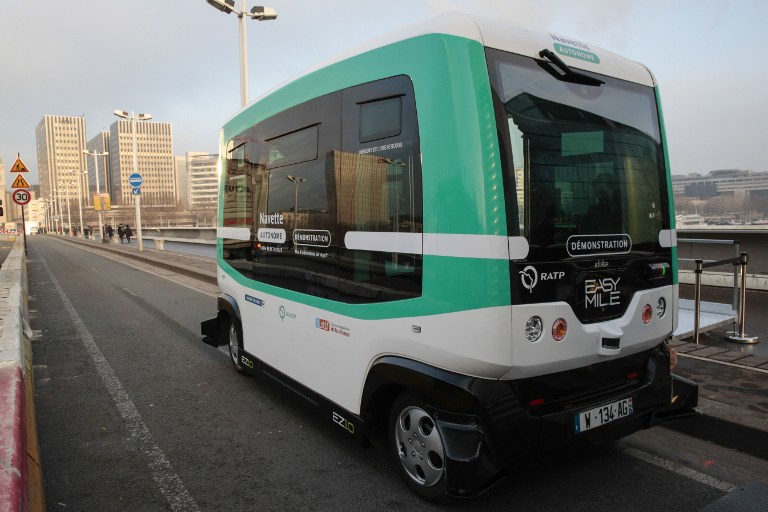
\includegraphics[width=\linewidth]{vect/intro/fig2/bus-auto}
		\vfill
		\textbf<2>{Autonomous driving}
	\end{minipage}
	}
	\uncover<3>{
	\begin{minipage}[t]{0.31\linewidth}
		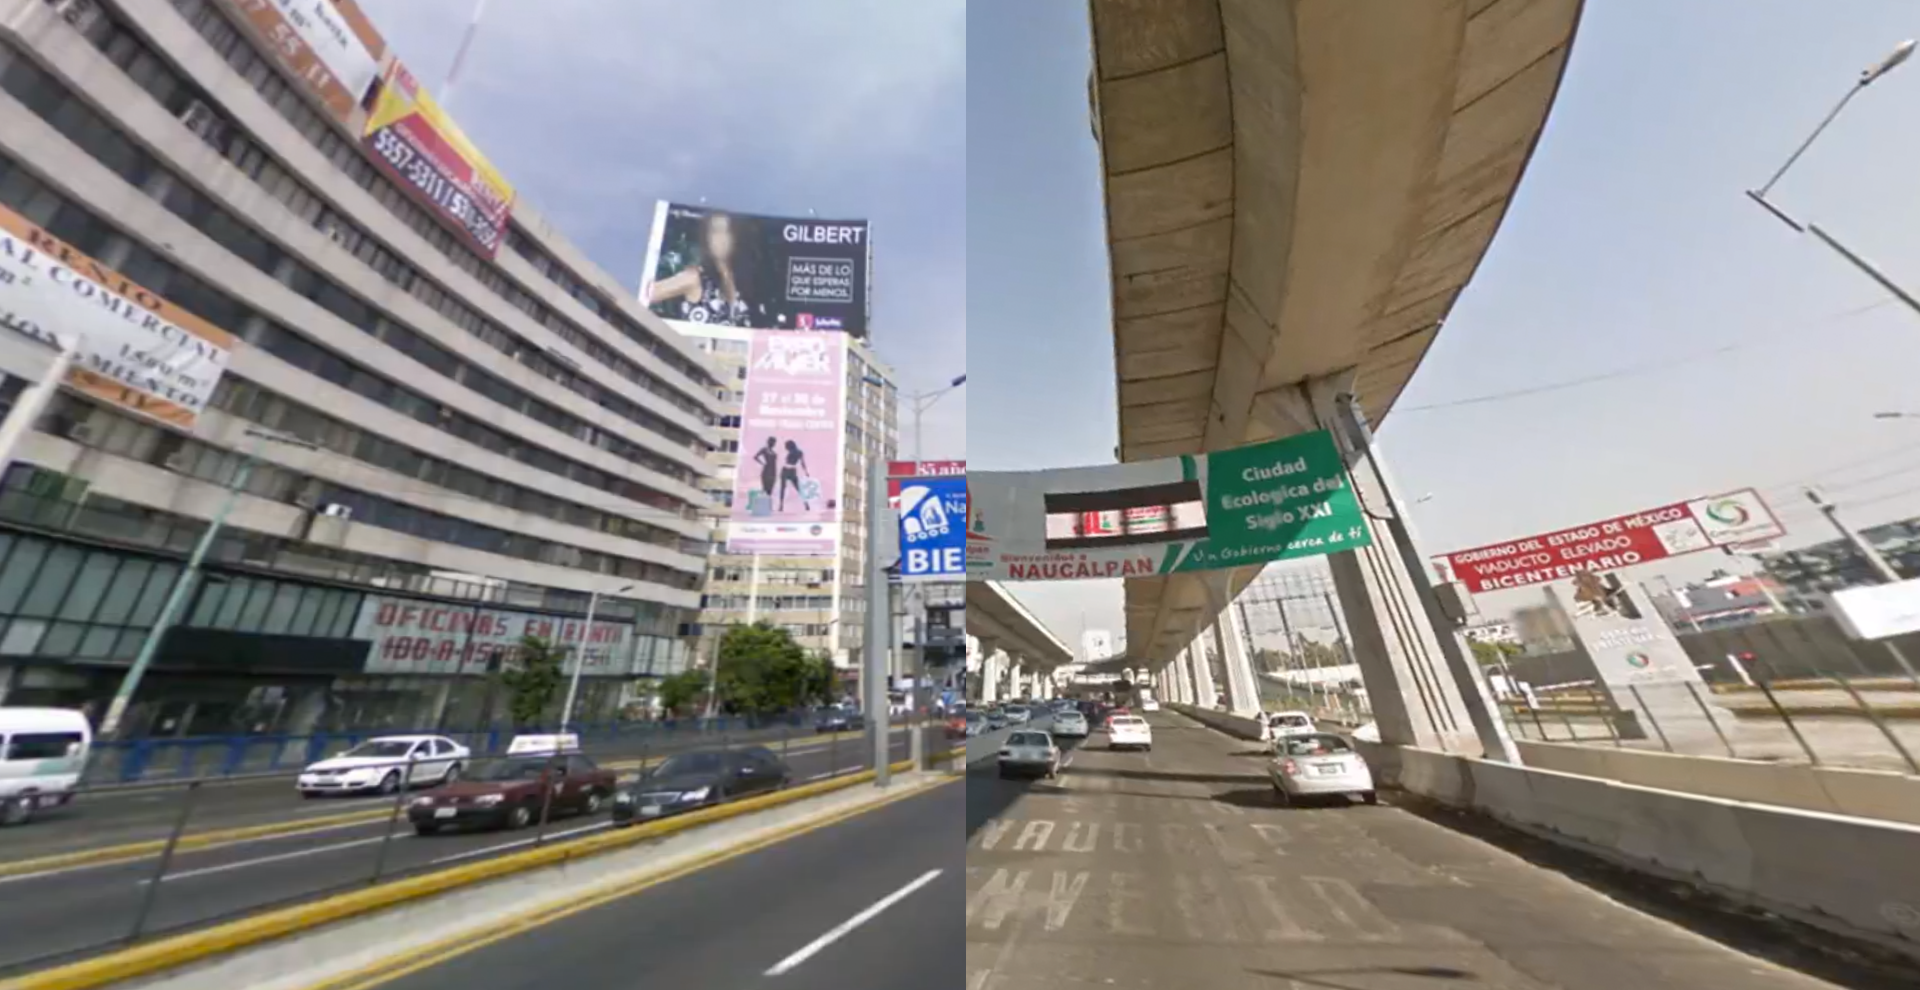
\includegraphics[width=\linewidth]{vect/intro/fig2/time-machine}
		\vfill
		\textbf<3>{Update of referential}
	\end{minipage}
	}
	}
\end{frame}

\begin{frame}{Image-retrieval}
	\only<1>
	{
	\begin{figure}[t]
		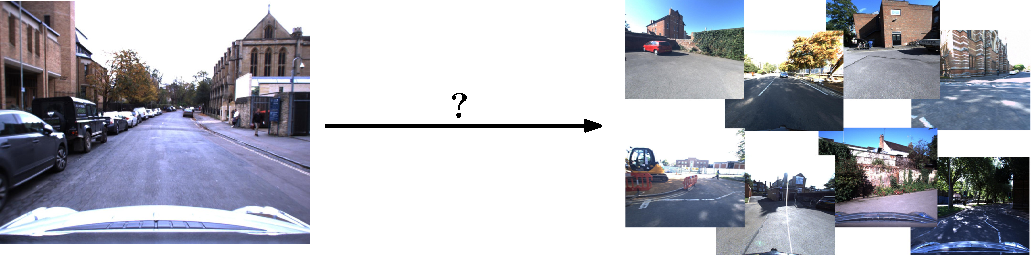
\includegraphics[width=0.8\linewidth]{vect/intro/fig3/cbir}
	\end{figure}
	\vfill	
	How to find the most similar image in a pool of candidates?
	}
	\only<2>
	{
	\begin{figure}[t]
		\centering
		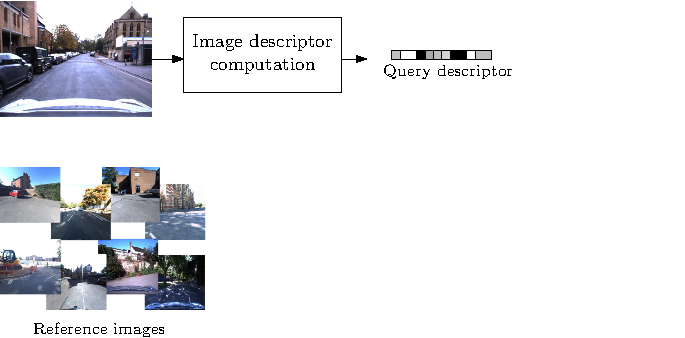
\includegraphics[width=0.8\linewidth]{vect/intro/fig3/1}
	\end{figure}
	\vfill	
	Compute a compact and discriminative descriptor.
	}
	\only<3>
	{
	\begin{figure}[t]
		\centering
		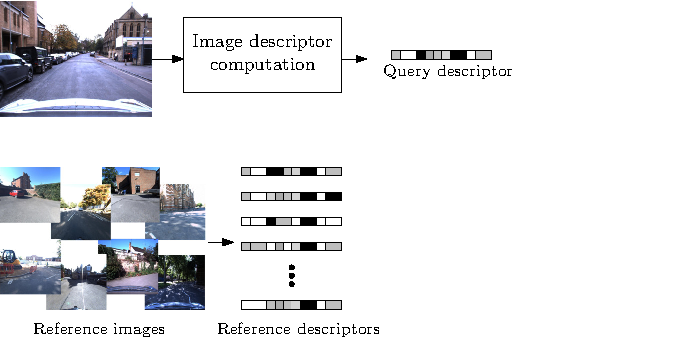
\includegraphics[width=0.8\linewidth]{vect/intro/fig3/2}
	\end{figure}
	\vfill	
	Compute descriptors of the reference data.
	}
	\only<4>
	{
	\begin{figure}[t]
		\centering
		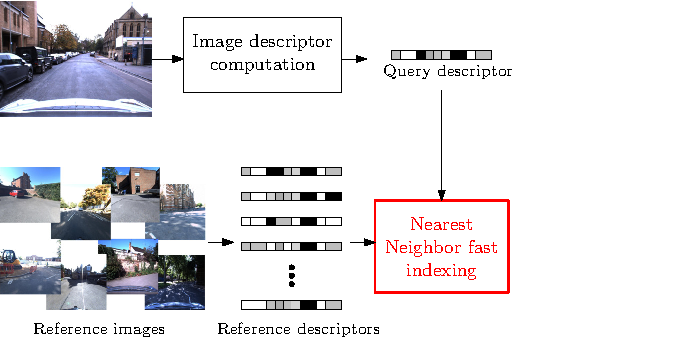
\includegraphics[width=0.8\linewidth]{vect/intro/fig3/3}
	\end{figure}
	\vfill	
	Compare descriptors with fast indexing method.
	}
	\only<5>
	{
	\begin{figure}[t]
		\centering
		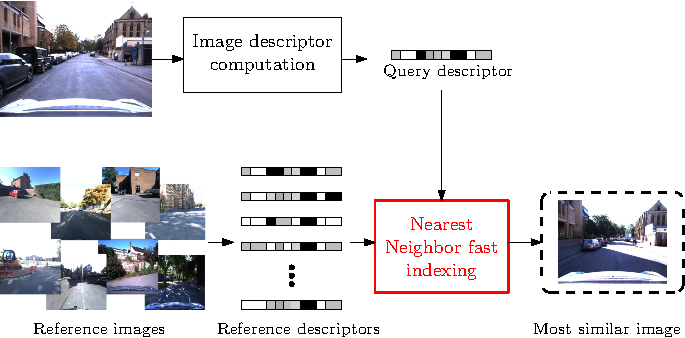
\includegraphics[width=0.8\linewidth]{vect/intro/fig3/4}
	\end{figure}
	\vfill	
	Retrieve reference candidate minimizing similarity score between descriptors.
	}
	\only<6>
	{
	\begin{figure}[t]
		\centering
		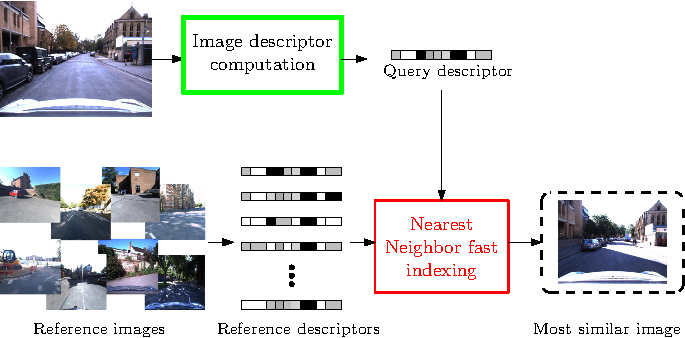
\includegraphics[width=0.8\linewidth]{vect/intro/fig3/5}
	\end{figure}
	\vfill	
	
	We introduce a new method to compute discriminative image descriptor.
	}
\end{frame}

\begin{frame}{Challenge in visual based localization}
\only<1>
	{
	\vfill
	\begin{figure}
		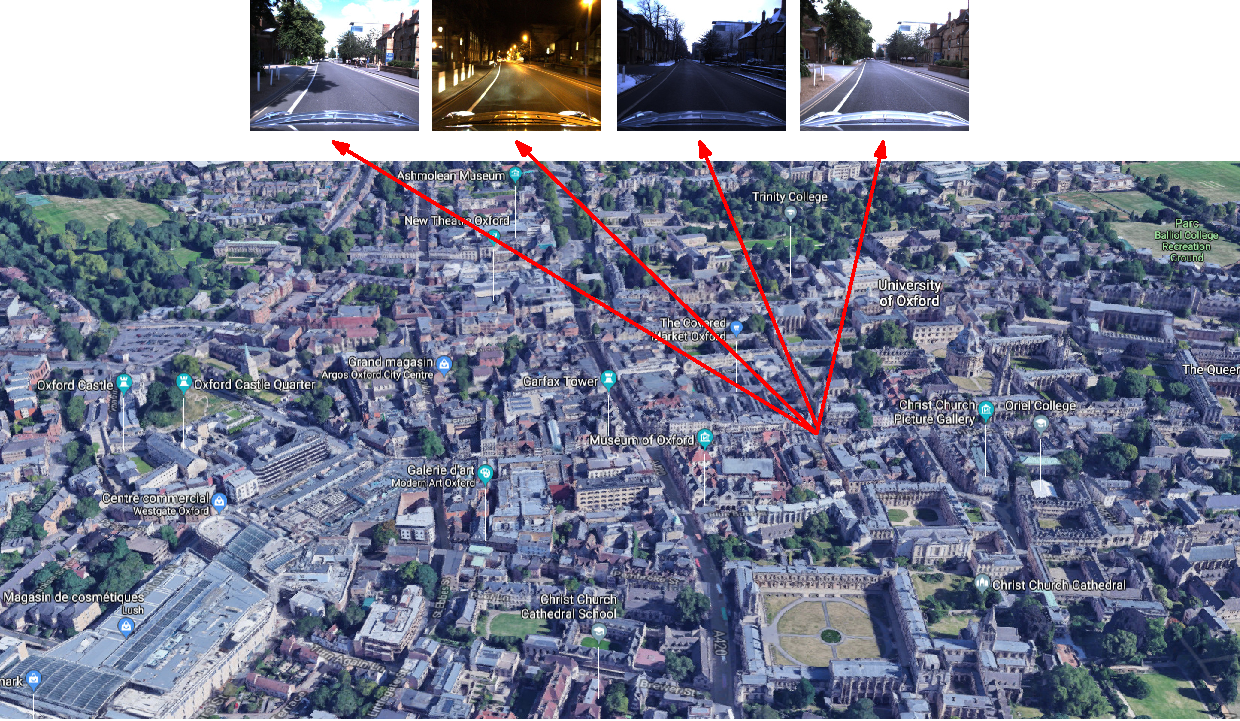
\includegraphics[width=0.8\linewidth]{vect/intro/fig4/1}
	\end{figure}
	\vfill	
	Drastic \textbf{visual changes} occur due to season/day-night cycles.
	}
	\only<2>
	{
	\vfill
	\begin{figure}
		\centering
		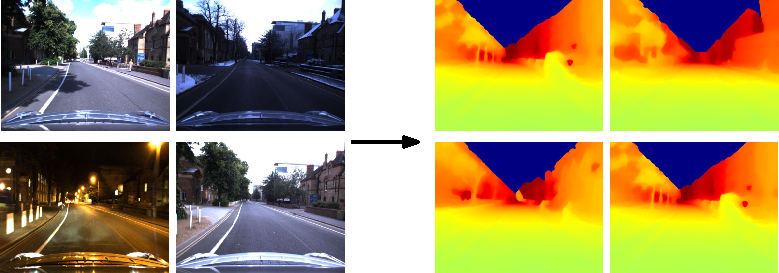
\includegraphics[width=0.8\linewidth]{vect/intro/fig4/2}
	\end{figure}
	\vfill	
	However, \textbf{geometric information} still remains the same.
	}
	\only<3>
	{
	\vfill
	\begin{figure}
		\centering
		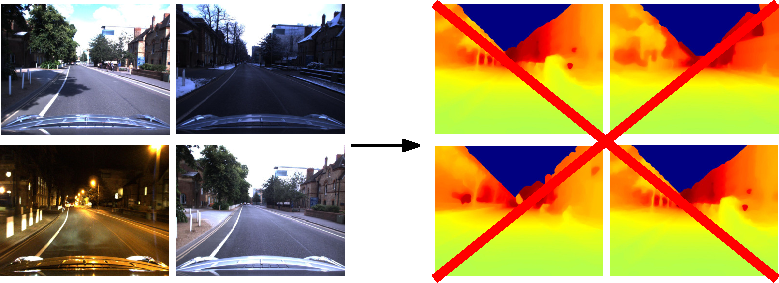
\includegraphics[width=0.8\linewidth]{vect/intro/fig4/3}
	\end{figure}
	\vfill	
	Unfortunately, geometric information is \textbf{not always available}.
	}
	\only<4>
	{
	\vfill
	\centering
	\begin{figure}
		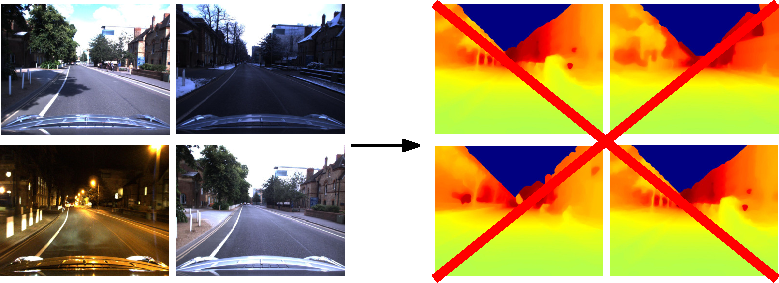
\includegraphics[width=0.6\linewidth]{vect/intro/fig4/3}
	\end{figure}
	\vfill	
	\textbf{How to use partial geometric information to improve image descriptor for localization?}
	}
\end{frame}
%
%
%\begin{frame}{Challenge in visual based localization}
%	Image retrieval is performed by measuring the similarity of low dimensional descriptors extracted from images.
%	\vfill
%	\begin{figure}
%		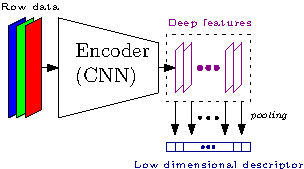
\includegraphics[width=0.5\linewidth]{vect/intro/Desc}
%		\caption{We use a CNN as trainable global image descriptor.}
%	\end{figure}
%	\vfill	
%	Global image descriptor can be trained with \textit{triplet loss} function\footfullcite{Arandjelovic2017}.
%\end{frame}
%
%\begin{frame}{Training a descriptor}
%	\begin{minipage}{0.49\linewidth}
%		\begin{minipage}[c]{0.26\linewidth}
%			\uncover<1->{\includegraphics[width=\linewidth]{im/intro/anchor.png}}
%			\vspace{0.1cm}
%			\uncover<2->{\includegraphics[width=\linewidth]{im/intro/positive.png}}
%			\vspace{0.1cm}
%			\uncover<3>{\includegraphics[width=\linewidth]{im/intro/negative.png}}
%		\end{minipage}
%		\begin{minipage}{0.7\linewidth}
%			\vfill
%			\begin{figure}
%				\centering
%				\includegraphics[width=\linewidth]{vect/intro/triplet_loss}
%			\end{figure}
%			\vfill
%		\end{minipage}
%	\end{minipage}
%	\begin{minipage}{0.48\linewidth}
%		\uncover<3>{
%			\begin{multline}
%				\label{eq:triplet_loss}
%				Loss_{triplet} = max\left( \norm{f(q) - f(q^+)}^2 - \right. \\
%				\left. \norm{f(q) - f(q^-)}^2 + \lambda, 0\right),
%			\end{multline}
%		}
%		\vfill
%		\only<1>{
%			\begin{align*}
%			with 
%			\begin{cases}
%					f(x) = \textnormal{descriptor of image $x$ } \\
%					q = \textnormal{query image} \\
%			\end{cases}
%			\end{align*}
%		}
%		\only<2>{
%			\begin{align*}
%			with 
%			\begin{cases}
%					f(x) = \textnormal{descriptor of image $x$ } \\
%					q = \textnormal{query image} \\
%					q^+ = \textnormal{positif example} \\
%			\end{cases}
%			\end{align*}
%		}
%		\only<3>{
%			\begin{align*}
%			with 
%			\begin{cases}
%					f(x) = \textnormal{descriptor of image $x$ } \\
%					q = \textnormal{query image} \\
%					q^+ = \textnormal{positif example} \\
%					q^- = \textnormal{negatif example} \\
%					\lambda = \textnormal{triplet loss margin} \\
%			\end{cases}
%			\end{align*}
%		}
%	\end{minipage}
%\end{frame}
%
%\begin{frame}{Handling multi-modal data}
%	We admit that we have multi-modal data only during the training step of our deep descriptor, and only RGB images at query time.
%	\vfill
%	\begin{block}{Proposed scenario}
%		\centering
%		\begin{tabular}{c | c}
%			\textbf{Training data type} & \textbf{Testing data type} \\
%			\hline
%			\textbf<1>{RGB + Depth} & \uncover<2->{\textbf<2>{RGB}}  \\
%		\end{tabular}
%	\end{block}
%	\begin{figure}[t]
%		\centering
%		\begin{minipage}[b]{0.65\linewidth}
%			\centering
%			{\footnotesize \textbf{Multi-modal} training dataset}	
%	
%			\includegraphics[width=0.50\linewidth]{im/intro/mod0.png}
%			\includegraphics[width=0.47\linewidth]{im/intro/mod1.png}
%		\end{minipage}
%		\uncover<2->{
%		\begin{minipage}[b]{0.32\linewidth}
%			\centering
%			{\footnotesize \textbf{Single modality} data at test time}
%	
%			\includegraphics[width=0.85\linewidth]{im/intro/q.jpg}
%		\end{minipage}
%		}
%	\end{figure}
%	\vfill
%	\uncover<3>{
%	\centering
%	\textbf{How to use extra-modalities to improve our image description?}
%	}
%\end{frame}